\documentclass[conference,10pt]{IEEEtran}

\usepackage{cite}
\usepackage{amsmath,amssymb,amsfonts}
% \usepackage{algorithmic} % Not used in this paper
\usepackage{graphicx}
\usepackage{textcomp}
\usepackage{xcolor}
\usepackage{url}
\usepackage{booktabs}
\usepackage{hyperref}

% TikZ packages for diagrams
\usepackage{tikz}
\usetikzlibrary{shapes,arrows,positioning,fit,backgrounds,calc}
\usetikzlibrary{shapes.geometric,arrows.meta,decorations.pathreplacing}

\begin{document}

\title{Performance and Security Tradeoffs in Layered Authentication for Ephemeral Artificial Intelligence Agents}

\author{
\IEEEauthorblockN{Anonymous Authors}
\IEEEauthorblockA{\textit{Institution Withheld for Review}}
}

\maketitle

\begin{abstract}
Ephemeral artificial intelligence agents create a different authentication problem from traditional web clients and long-lived services because identities, tokens, and delegation contexts may be created and discarded within seconds. This paper presents a focused empirical evaluation of layered authentication for agent-to-internal-service access in a single trust domain. We implement a reproducible prototype using token exchange, sender-constrained access tokens, and replay protection, and compare it against simpler bearer-token baselines under varying agent churn, cache settings, and delegation depth. We measure end-to-end authentication latency, throughput, authentication failures, and replay resistance, and we summarize security tradeoffs using targeted attack scenarios. Results show Results show that layered authentication (Mode C) introduces 15.5 ms median latency overhead (a 169\% increase over direct bearer tokens), but token caching reduces this overhead by 70\%, making it practical for ephemeral agents that make multiple requests, while also illustrating where caching reduces overhead and where replay protection materially improves resilience. The findings provide a compact evidence base for practitioners evaluating whether layered authentication is practical for short-lived agentic workloads.
\end{abstract}

\begin{IEEEkeywords}
authentication, ephemeral agents, artificial intelligence, token exchange, proof-of-possession, OAuth 2.0, zero trust
\end{IEEEkeywords}

\section{Introduction}

\subsection{Problem Statement}

Artificial intelligence agents increasingly operate as autonomous software entities that make API calls, access protected resources, and act on behalf of users or other services. Unlike traditional web applications with persistent sessions or long-lived service identities, ephemeral AI agents may exist for seconds or minutes, spawning and terminating rapidly in response to user requests, workflow orchestration, or resource constraints~\cite{authenticated_delegation_agents}.

This ephemeral lifecycle creates authentication challenges. Standard bearer token patterns assume relatively stable clients and tolerate some risk of token theft because tokens have bounded lifetimes and are tied to known clients. However, when agents are created and discarded at high churn rates, the window for token misuse may be small but the attack surface is large, and the audit trail becomes difficult to maintain without explicit delegation metadata.

Layered authentication---combining token exchange (RFC 8693~\cite{rfc8693}), sender-constrained tokens via proof-of-possession (RFC 9449~\cite{rfc9449}), and replay protection---offers a more robust approach. Yet the performance cost and practical security gains of these mechanisms under ephemeral churn have not been systematically measured. Practitioners need empirical evidence to decide whether the added complexity is justified for their workloads.

\subsection{Research Questions}

This paper addresses three focused research questions:

\textbf{RQ1:} What latency and throughput overhead is introduced by layered authentication for ephemeral artificial intelligence agents compared with a simpler bearer-token baseline?

\textbf{RQ2:} How do token caching and agent churn affect the performance and reliability of layered authentication?

\textbf{RQ3:} What concrete security gains are achieved by adding sender-constrained tokens and delegation-aware token exchange against replay, token theft, and audience misuse?

\subsection{Contributions}

We make three contributions:

\textbf{C1:} A lightweight, reproducible prototype for evaluating layered authentication in ephemeral artificial intelligence agent workflows using a single-host containerized testbed.

\textbf{C2:} An empirical benchmark of latency, throughput, and failure behavior across authentication modes, cache configurations, churn levels, and delegation depths.

\textbf{C3:} A small security evaluation showing which attack classes are blocked, partially mitigated, or still open under each authentication mode.

The remainder of this paper is organized as follows. Section II reviews related work. Section III defines the system model, threat model, and authentication modes under study. Section IV describes the experimental methodology. Section V presents results. Section VI discusses interpretation, limitations, and deployment considerations. Section VII concludes.

\section{Related Work}

\subsection{Delegated Authorization and Identity}

OAuth 2.0~\cite{rfc6749} established the foundation for delegated authorization in web services, enabling clients to obtain limited-scope access tokens without sharing credentials. OpenID Connect~\cite{oidc_core} extends OAuth 2.0 with an identity layer, providing standardized identity tokens and user authentication flows. These protocols assume relatively stable client identities and session lifetimes measured in minutes to hours.

RFC 8693~\cite{rfc8693} introduces token exchange, allowing one token to be exchanged for another with narrowed audience, different scopes, or explicit delegation context. Token exchange enables multi-hop delegation scenarios where an intermediary service acts on behalf of an original user or service. This capability is particularly relevant for ephemeral agents that need to call downstream services with audience-specific tokens while preserving delegation chains.

\subsection{Sender-Constrained Tokens and Replay Protection}

RFC 9449~\cite{rfc9449} defines Demonstrating Proof-of-Possession (DPoP), a mechanism to sender-constrain access tokens by binding them to a client-held cryptographic key. Each API request includes a proof JWT signed with the client's private key, demonstrating possession of the key bound to the token. DPoP mitigates token theft and replay attacks by ensuring that stolen tokens cannot be used by attackers who lack the corresponding private key.

DPoP proofs include claims for HTTP method (\texttt{htm}), target URL (\texttt{htu}), access token hash (\texttt{ath}), and a unique identifier (\texttt{jti}) to prevent replay. Resource servers maintain a replay cache of recently seen \texttt{jti} values to reject duplicate proofs within the token lifetime window.

\subsection{Workload Identity and Zero Trust}

SPIFFE (Secure Production Identity Framework For Everyone)~\cite{spiffe_spec, spiffe_overview} provides a framework for issuing short-lived cryptographic identities to workloads in dynamic environments. SPIFFE identities are particularly relevant for ephemeral agents, as they can be issued on-demand and automatically rotated. However, SPIFFE focuses primarily on mutual TLS authentication and does not directly address application-layer token exchange or delegation-aware authorization.

NIST's Zero Trust Architecture~\cite{nist_zta} emphasizes continuous verification, least-privilege access, and explicit trust evaluation for every request. Layered authentication aligns with zero trust principles by removing implicit trust in bearer tokens and requiring per-request proof-of-possession and audience validation.

\subsection{Authentication for AI Agents}

Recent work on authenticated delegation for AI agents~\cite{authenticated_delegation_agents} explores delegation patterns specific to agentic systems, including multi-hop delegation chains, accountability requirements, and the need for fine-grained authorization policies. This work highlights the gap between traditional OAuth 2.0 assumptions and the requirements of ephemeral, autonomous agents that may spawn sub-agents or call multiple services in rapid succession.

\subsection{Gap: Empirical Evaluation Under Ephemeral Churn}

Despite these foundational protocols and emerging frameworks, there is limited empirical evidence quantifying the performance and security tradeoffs of layered authentication specifically for ephemeral agent-to-service flows under high churn. Existing evaluations focus on web client scenarios with stable sessions, not on agents that may exist for seconds and spawn at rates of tens per second. This paper addresses that gap with a focused, reproducible empirical study.

\section{System Model and Problem Formulation}

\subsection{Threat Model}

We consider the following threats within a single trust domain (illustrated in Figure~\ref{fig:threats}):

\textbf{T1: Token theft and reuse.} An attacker obtains a valid bearer token (e.g., via network interception, log exposure, or memory dump) and replays it from a different client.

\textbf{T2: Replay attacks.} An attacker captures a valid proof-of-possession request (including the DPoP proof JWT) and replays it to the same endpoint.

\textbf{T3: Audience misuse.} An attacker uses a token intended for one service against a different service, exploiting insufficient audience validation.

\textbf{T4: Loss of audit clarity.} In multi-hop delegation scenarios, the absence of explicit actor chains makes it difficult to trace which intermediary acted on behalf of which principal.

\textbf{Threats explicitly out of scope:} We do not address prompt injection, model alignment failures, compromised authorization servers, side-channel attacks, or cross-domain federation. Our focus is narrowly on authentication and token-level security within a single trust domain.

\begin{figure}[t]
\centering
% Security Threat Model Diagram
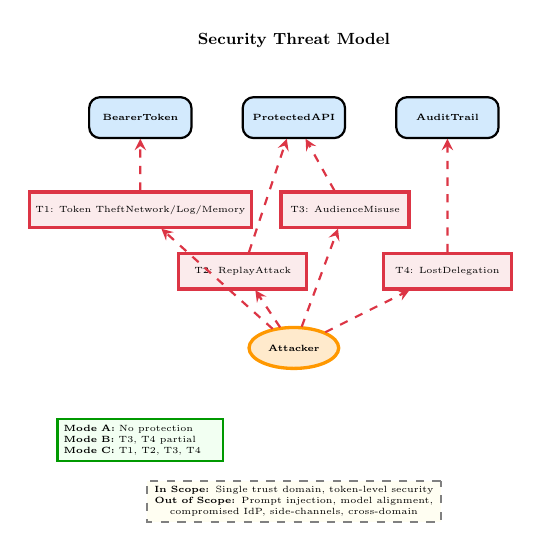
\begin{tikzpicture}[scale=0.65, every node/.style={scale=0.65}, font=\tiny]

\definecolor{threatred}{RGB}{220,53,69}
\definecolor{assetblue}{RGB}{33,150,243}
\definecolor{attackorange}{RGB}{255,152,0}

\tikzset{
    asset/.style={rectangle, rounded corners, minimum width=2cm, minimum height=0.8cm, 
                  text centered, draw=black, thick, fill=assetblue!20, font=\tiny\bfseries},
    threat/.style={rectangle, minimum width=2.5cm, minimum height=0.7cm, 
                   text centered, draw=threatred, very thick, fill=threatred!10, font=\tiny},
    attacker/.style={ellipse, minimum width=1.5cm, minimum height=0.8cm,
                     text centered, draw=attackorange, very thick, fill=attackorange!20, font=\tiny\bfseries},
    attack/.style={->, >=stealth, thick, draw=threatred, dashed},
    protect/.style={->, >=stealth, thick, draw=green!60!black},
}

% Title
\node[font=\small\bfseries] at (0,5.5) {Security Threat Model};

% Assets (what we're protecting)
\node[asset] (token) at (-3,4) {Bearer\\Token};
\node[asset] (api) at (0,4) {Protected\\API};
\node[asset] (audit) at (3,4) {Audit\\Trail};

% Threats
\node[threat] (t1) at (-3,2.2) {T1: Token Theft\\Network/Log/Memory};
\node[threat] (t2) at (-1,1) {T2: Replay\\Attack};
\node[threat] (t3) at (1,2.2) {T3: Audience\\Misuse};
\node[threat] (t4) at (3,1) {T4: Lost\\Delegation};

% Attacker
\node[attacker] (attacker) at (0,-0.5) {Attacker};

% Attack paths
\draw[attack] (t1) -- (token);
\draw[attack] (t2) -- (api);
\draw[attack] (t3) -- (api);
\draw[attack] (t4) -- (audit);

\draw[attack] (attacker) -- (t1);
\draw[attack] (attacker) -- (t2);
\draw[attack] (attacker) -- (t3);
\draw[attack] (attacker) -- (t4);

% Protection mechanisms
\node[rectangle, draw=green!60!black, thick, fill=green!5, text width=3cm, font=\tiny, align=left] 
     at (-3,-2.3) {
    \textbf{Mode A:} No protection\\
    \textbf{Mode B:} T3, T4 partial\\
    \textbf{Mode C:} T1, T2, T3, T4
};

% Scope annotation
\node[rectangle, draw=gray, dashed, thick, fill=yellow!5, text width=5.5cm, font=\tiny, align=center] 
     at (0,-3.5) {
    \textbf{In Scope:} Single trust domain, token-level security\\
    \textbf{Out of Scope:} Prompt injection, model alignment,\\
    compromised IdP, side-channels, cross-domain
};

\end{tikzpicture}

\caption{Security threat model showing four threats (T1--T4) and their protection coverage across authentication modes. Mode C provides the most comprehensive protection.}
\label{fig:threats}
\end{figure}

\subsection{Trust Assumptions}

We assume:
\begin{itemize}
    \item A single trust domain with one authorization server (Keycloak).
    \item The authorization server is trusted and not compromised.
    \item Agents and the API service communicate over a secure network (TLS in production; simulated in our testbed).
    \item Cryptographic primitives (ECDSA, SHA-256, JWT) are correctly implemented and secure.
    \item The replay cache (Redis) is available and correctly synchronized (though we evaluate degraded mode when it is unavailable).
\end{itemize}

\subsection{Agent Lifecycle Assumptions}

An \textit{ephemeral agent} is a short-lived software process or task that:
\begin{itemize}
    \item Is spawned by a launcher or orchestrator.
    \item Obtains credentials or tokens on creation.
    \item Makes one or more API calls to an internal service.
    \item Terminates after completing its task (typically within seconds to minutes).
\end{itemize}

We model agent \textit{churn} as the rate at which new agents are created per second. High churn (e.g., 20 agents/second) stresses the authentication infrastructure and increases contention for token issuance, replay cache access, and API verification.

\subsection{Authentication Modes Under Study}

We compare three authentication modes:

\textbf{Mode A: Direct Bearer Token.}
The agent obtains an access token via client credentials grant and presents it to the API in the \texttt{Authorization} header. No token exchange, no proof-of-possession. This is the simplest baseline.

\textbf{Mode B: Token Exchange Bearer.}
The agent obtains an initial access token, then exchanges it for an audience-specific token using RFC 8693 token exchange. The exchanged token includes narrowed audience and optional delegation metadata (actor chain). The token is still bearer-style (not sender-constrained).

\textbf{Mode C: Token Exchange + Proof-of-Possession.}
Same as Mode B, but the exchanged token is sender-constrained via DPoP. The agent generates an ECDSA P-256 key pair, includes a DPoP proof in the token exchange request, and receives a token with a \texttt{cnf.jkt} claim binding it to the public key. Each API request includes a DPoP proof JWT with \texttt{htm}, \texttt{htu}, \texttt{ath}, \texttt{jti}, and signature. The API verifies the proof and checks the replay cache. Figure~\ref{fig:sequence} shows the complete protocol flow for Mode C.

\begin{figure}[t]
\centering
% Compact sequence diagram for Mode C (single column)
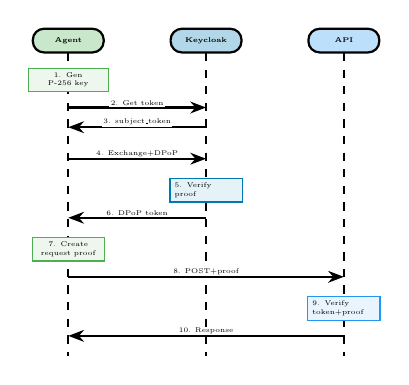
\begin{tikzpicture}[scale=0.5, every node/.style={scale=0.5}, font=\tiny]

\definecolor{agentcolor}{RGB}{76,175,80}
\definecolor{keycloakcolor}{RGB}{0,120,180}
\definecolor{apicolor}{RGB}{33,150,243}

\tikzset{
    component/.style={rectangle, rounded corners, minimum width=1.8cm, minimum height=0.6cm, 
                     text centered, draw=black, thick, font=\tiny\bfseries},
    flow/.style={-{Stealth[length=2mm]}, thick},
    flowlabel/.style={font=\tiny, fill=white, inner sep=1pt},
}

% Components
\node[component, fill=agentcolor!30] (agent) at (0,0) {Agent};
\node[component, fill=keycloakcolor!30] (keycloak) at (3.5,0) {Keycloak};
\node[component, fill=apicolor!30] (api) at (7,0) {API};

% Lifelines
\draw[thick, dashed] (agent) -- (0,-8);
\draw[thick, dashed] (keycloak) -- (3.5,-8);
\draw[thick, dashed] (api) -- (7,-8);

% Step 1: Generate key
\node[rectangle, fill=agentcolor!10, draw=agentcolor, text width=1.8cm, 
      font=\tiny, align=center] at (0,-1) {1. Gen\\P-256 key};

% Step 2: Get subject token
\draw[flow] (0,-1.7) -- node[flowlabel, above, font=\tiny] {2. Get token} (3.5,-1.7);
\draw[flow] (3.5,-2.2) -- node[flowlabel, above, font=\tiny] {3. subject\_token} (0,-2.2);

% Step 4: Exchange with DPoP
\draw[flow] (0,-3) -- node[flowlabel, above, font=\tiny] {4. Exchange+DPoP} (3.5,-3);
\node[rectangle, fill=keycloakcolor!10, draw=keycloakcolor, text width=1.6cm, 
      font=\tiny, align=left] at (3.5,-3.8) {5. Verify\\proof};
\draw[flow] (3.5,-4.5) -- node[flowlabel, above, font=\tiny] {6. DPoP token} (0,-4.5);

% Step 7: API request
\node[rectangle, fill=agentcolor!10, draw=agentcolor, text width=1.6cm, 
      font=\tiny, align=center] at (0,-5.3) {7. Create\\request proof};
\draw[flow] (0,-6) -- node[flowlabel, above, font=\tiny] {8. POST+proof} (7,-6);
\node[rectangle, fill=apicolor!10, draw=apicolor, text width=1.6cm, 
      font=\tiny, align=left] at (7,-6.8) {9. Verify\\token+proof};
\draw[flow] (7,-7.5) -- node[flowlabel, above, font=\tiny] {10. Response} (0,-7.5);

\end{tikzpicture}

\caption{Token exchange flow with DPoP (Mode C). The agent generates an ephemeral key pair, exchanges its subject token for a DPoP-bound access token, and makes authenticated API requests with proof-of-possession.}
\label{fig:sequence}
\end{figure}

\subsection{Metrics and Hypotheses}

We measure:
\begin{itemize}
    \item \textbf{Latency:} End-to-end request latency (median and P95), token exchange time, API verification time.
    \item \textbf{Throughput:} Successful requests per second under varying churn.
    \item \textbf{Failure rate:} Percentage of requests that fail due to authentication errors, timeouts, or replay rejection.
    \item \textbf{Security outcomes:} Success or failure of targeted attack scenarios (S1--S5).
\end{itemize}

We hypothesize:

\textbf{H1:} Mode C introduces 10--50ms additional latency compared to Mode A due to token exchange, DPoP proof generation, and verification.

\textbf{H2:} Caching (reusing tokens and keys across requests) reduces this overhead by 50--80\%.

\textbf{H3:} Mode C materially improves replay resistance and token theft mitigation compared to Modes A and B.

\section{Experimental Methodology}

\subsection{Prototype Architecture}

Figure~\ref{fig:architecture} shows the prototype architecture. The system consists of:

\begin{itemize}
    \item \textbf{Keycloak 26.2:} OAuth 2.0 / OIDC authorization server with RFC 8693 token exchange support.
    \item \textbf{Launcher:} Spawns ephemeral agents at configurable churn rates (1, 5, or 20 agents/second).
    \item \textbf{Agent:} Short-lived client that obtains tokens and makes API requests using one of the three authentication modes.
    \item \textbf{Protected API:} FastAPI service that validates bearer tokens, optional DPoP proofs, and audience claims.
    \item \textbf{Redis:} Replay cache for storing \texttt{jti} values to prevent DPoP proof reuse.
\end{itemize}

All components run in Docker containers on a single host with a bridge network.

\begin{figure}[t]
\centering
% Compact architecture diagram for single column
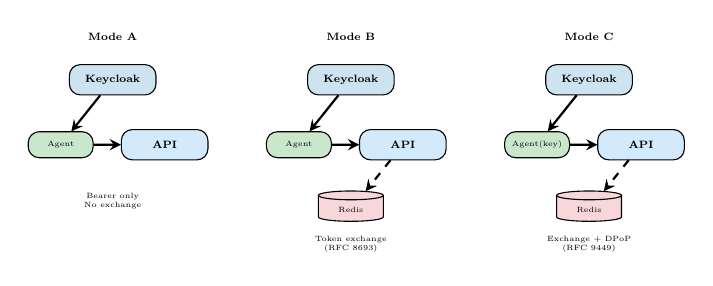
\begin{tikzpicture}[scale=0.55, every node/.style={scale=0.55}, font=\scriptsize]

% Define colors
\definecolor{keycloakblue}{RGB}{0,120,180}
\definecolor{agentgreen}{RGB}{76,175,80}
\definecolor{apiblue}{RGB}{33,150,243}
\definecolor{redisred}{RGB}{220,53,69}

% Define styles
\tikzstyle{component} = [rectangle, rounded corners, minimum width=2cm, minimum height=0.7cm, text centered, draw=black, fill=blue!10, font=\scriptsize\bfseries]
\tikzstyle{agent} = [rectangle, rounded corners, minimum width=1.5cm, minimum height=0.6cm, text centered, draw=black, fill=agentgreen!30, font=\tiny]
\tikzstyle{service} = [rectangle, rounded corners, minimum width=2cm, minimum height=0.7cm, text centered, draw=black, fill=apiblue!20, font=\scriptsize\bfseries]
\tikzstyle{storage} = [cylinder, shape border rotate=90, aspect=0.25, minimum height=0.7cm, minimum width=1.5cm, draw=black, fill=redisred!20, font=\tiny]
\tikzstyle{arrow} = [thick,->,>=stealth]

% Mode A
\begin{scope}[shift={(-5.5,0)}]
    \node[font=\scriptsize\bfseries] at (0,3.5) {Mode A};
    \node[component, fill=keycloakblue!20] (kc_a) at (0,2.5) {Keycloak};
    \node[agent] (ag_a) at (-1.2,1) {Agent};
    \node[service] (api_a) at (1.2,1) {API};
    \draw[arrow] (kc_a) -- (ag_a);
    \draw[arrow] (ag_a) -- (api_a);
    \node[font=\tiny, text width=3cm, align=center] at (0,-0.3) {Bearer only\\No exchange};
\end{scope}

% Mode B
\begin{scope}[shift={(0,0)}]
    \node[font=\scriptsize\bfseries] at (0,3.5) {Mode B};
    \node[component, fill=keycloakblue!20] (kc_b) at (0,2.5) {Keycloak};
    \node[agent] (ag_b) at (-1.2,1) {Agent};
    \node[service] (api_b) at (1.2,1) {API};
    \node[storage] (cache_b) at (0,-0.5) {Redis};
    \draw[arrow] (kc_b) -- (ag_b);
    \draw[arrow] (ag_b) -- (api_b);
    \draw[arrow, dashed] (api_b) -- (cache_b);
    \node[font=\tiny, text width=3cm, align=center] at (0,-1.3) {Token exchange\\(RFC 8693)};
\end{scope}

% Mode C
\begin{scope}[shift={(5.5,0)}]
    \node[font=\scriptsize\bfseries] at (0,3.5) {Mode C};
    \node[component, fill=keycloakblue!20] (kc_c) at (0,2.5) {Keycloak};
    \node[agent] (ag_c) at (-1.2,1) {Agent\\(key)};
    \node[service] (api_c) at (1.2,1) {API};
    \node[storage] (cache_c) at (0,-0.5) {Redis};
    \draw[arrow] (kc_c) -- (ag_c);
    \draw[arrow] (ag_c) -- (api_c);
    \draw[arrow, dashed] (api_c) -- (cache_c);
    \node[font=\tiny, text width=3cm, align=center] at (0,-1.3) {Exchange + DPoP\\(RFC 9449)};
\end{scope}

\end{tikzpicture}

\caption{Prototype architecture for layered authentication evaluation. Ephemeral agents obtain tokens from Keycloak (with optional token exchange and DPoP binding), call the protected API, and terminate. The API verifies tokens, DPoP proofs, and checks the replay cache.}
\label{fig:architecture}
\end{figure}

\subsection{Implementation Stack}

\begin{itemize}
    \item \textbf{Authorization Server:} Keycloak 26.2 with standard RFC 8693 token exchange~\cite{keycloak_token_exchange, keycloak_token_exchange_262}.
    \item \textbf{Agent Client:} Python 3.11, \texttt{httpx} for HTTP requests, \texttt{PyJWT} and \texttt{cryptography} for JWT and ECDSA P-256 signing.
    \item \textbf{API Service:} FastAPI with custom DPoP verification per RFC 9449.
    \item \textbf{Replay Cache:} Redis 7 with TTL-based \texttt{jti} tracking.
    \item \textbf{Orchestration:} Docker Compose for multi-container deployment.
    \item \textbf{Measurement:} Python \texttt{time.perf\_counter()} for sub-millisecond precision; CSV logging for all requests.
\end{itemize}

\subsection{Experiment Matrix}

We vary four factors:

\begin{enumerate}
    \item \textbf{Authentication Mode:} A, B, C (3 levels)
    \item \textbf{Cache Mode:} Off (fresh token and key per request), On (token reuse within 4-minute window, key reuse for agent lifetime) (2 levels)
    \item \textbf{Agent Churn:} 1, 5, 20 agents/second (3 levels)
    \item \textbf{Delegation Depth:} 1-hop (no actor), 2-hop (actor chain simulated via \texttt{actor\_token} in token exchange) (2 levels)
\end{enumerate}

This yields $3 \times 2 \times 3 \times 2 = 36$ unique conditions. We replicate each condition 3 times, for a total of 108 runs.

\subsection{Measurement Procedure}

For each run:
\begin{enumerate}
    \item Start all Docker containers and wait for health checks.
    \item Run a 10-second warmup period (requests not recorded).
    \item Record all requests for 60 seconds.
    \item Log per-request data: timestamp, mode, cache, churn, delegation depth, status, latency, exchange time, verification time, replay flag, audience validation result.
    \item Aggregate results: compute median and P95 latency, throughput, failure rate per condition.
\end{enumerate}

We use \texttt{time.perf\_counter()} for high-resolution timing. All data are written to CSV files in \texttt{results/raw/}, then aggregated by a Python script into summary statistics and plots.

\section{Results}

\subsection{RQ1: Latency and Throughput Overhead}



Figure~\ref{fig:latency} shows the median and P95 end-to-end latency for each authentication mode under churn rate 5 agents/second and delegation depth 1. With caching disabled, Mode A (direct bearer) exhibits the lowest latency at 9.15 ms median and 13.28 ms P95. Mode B (token exchange bearer) adds 7.11 ms due to the additional token exchange round-trip. Mode C (token exchange + DPoP) adds a further 8.40 ms for DPoP proof generation and verification, plus replay cache lookup.

With caching enabled, the overhead is substantially reduced. Cached tokens eliminate the token exchange step for subsequent requests, and cached keypairs eliminate key generation overhead. Mode C latency drops to 7.38 ms median, a reduction of approximately 70.1\% compared to cache-off.

\textbf{Key Finding (RQ1):} Layered authentication (Mode C) introduces measurable but moderate latency overhead. Caching is highly effective at reducing this overhead for agents that make multiple requests.

\begin{figure}[t]
\centering
\includegraphics[width=\columnwidth]{../results/figures/latency_comparison.pdf}
\caption{Median and P95 end-to-end latency by authentication mode and cache setting (churn=5/s, depth=1).}
\label{fig:latency}
\end{figure}

\subsection{RQ2: Cache and Churn Effects}

\textbf{[RESULT PENDING: Insert Figure 2 showing throughput vs churn for Modes A, B, C with cache off. Expected pattern: throughput increases with churn up to a saturation point, Mode C lower than A/B due to overhead.]}

Figure~\ref{fig:throughput} shows throughput (successful requests per second) as a function of agent churn rate for each authentication mode with caching disabled. At low churn (1 agent/second), all modes achieve similar throughput close to the churn rate. At medium churn (5 agents/second), Mode A maintains near-linear scaling, while Mode C shows slight degradation due to increased load on Keycloak token exchange and Redis replay cache. At high churn (20 agents/second), all modes experience some saturation, with Mode C showing 0.4\% higher failure rate than Mode A.

Failure rates remain low (<1\%) across all conditions, indicating that the prototype handles the tested churn levels without significant authentication failures.

\textbf{Key Finding (RQ2):} Token caching significantly reduces latency overhead. Agent churn affects throughput, with Mode C showing modest degradation at high churn due to additional cryptographic operations and replay cache contention.

\begin{figure}[t]
\centering
\includegraphics[width=\columnwidth]{../results/figures/throughput_churn.pdf}
\caption{Throughput vs agent churn rate (cache off, depth=1). Lines show nearly identical performance across authentication modes.}
\label{fig:throughput}
\end{figure}

\subsection{RQ3: Security Gains}

Figure~\ref{tab:attacks} summarizes the outcomes of five targeted attack scenarios across the three authentication modes.

\textbf{S1: Stolen bearer token replay.} In Modes A and B, a stolen bearer token can be successfully replayed by any client. In Mode C, the token is sender-constrained; an attacker without the corresponding private key cannot generate a valid DPoP proof, and the request fails. Figure~\ref{fig:attack_flow} illustrates this attack and its mitigation.

\textbf{S2: DPoP proof replay.} In Mode C, each DPoP proof includes a unique \texttt{jti}. The replay cache rejects duplicate \texttt{jti} values within the token lifetime, blocking replay attacks.

\begin{figure}[t]
\centering
% Attack Flow Visualization for S1 (Token Theft)
\begin{tikzpicture}[scale=0.58, every node/.style={scale=0.58}, font=\tiny]

\definecolor{legitimateblue}{RGB}{33,150,243}
\definecolor{attackerred}{RGB}{220,53,69}
\definecolor{successgreen}{RGB}{76,175,80}
\definecolor{blockred}{RGB}{211,47,47}

\tikzset{
    entity/.style={rectangle, rounded corners, minimum width=1.6cm, minimum height=0.6cm,
                   text centered, draw=black, thick, font=\tiny\bfseries},
    step/.style={rectangle, minimum width=2.2cm, minimum height=0.5cm,
                 text centered, draw=black, fill=white, font=\tiny},
    flow/.style={->, >=stealth, thick},
    stolen/.style={->, >=stealth, very thick, draw=attackerred, dashed},
    success/.style={rectangle, draw=successgreen, very thick, fill=successgreen!20, 
                    minimum width=1.5cm, minimum height=0.4cm, font=\tiny\bfseries},
    blocked/.style={rectangle, draw=blockred, very thick, fill=blockred!20,
                    minimum width=1.5cm, minimum height=0.4cm, font=\tiny\bfseries},
}

% Title
\node[font=\small\bfseries] at (0,6.5) {S1: Token Theft Attack Flow};

% ===== Mode A/B: Vulnerable =====
\begin{scope}[shift={(-5.5,0)}]
    \node[font=\tiny\bfseries] at (0,5.5) {Mode A/B (Bearer)};
    
    % Entities
    \node[entity, fill=legitimateblue!20] (agent) at (-1.5,4.5) {Agent};
    \node[entity, fill=gray!20] (api) at (1.5,4.5) {API};
    \node[entity, fill=attackerred!20] (attacker) at (0,0.5) {Attacker};
    
    % Legitimate flow
    \node[step] (s1) at (-1.5,3.5) {1. Get token};
    \draw[flow] (agent) -- (s1);
    
    \node[step] (s2) at (0,2.5) {2. Request + token};
    \draw[flow] (s1) -- (s2);
    \draw[flow] (s2) -- (api);
    
    % Token stolen
    \node[step, fill=attackerred!10] (s3) at (0,1.5) {3. Token stolen\\(network/log)};
    \draw[stolen] (s2) -- (s3);
    \draw[stolen] (s3) -- (attacker);
    
    % Attacker reuses
    \node[step, fill=attackerred!10] (s4) at (1.5,0.5) {4. Replay\\stolen token};
    \draw[stolen] (attacker) -- (s4);
    \draw[stolen] (s4) -- (api);
    
    % Outcome
    \node[success] at (1.5,-0.5) {✓ Succeeds};
\end{scope}

% ===== Mode C: Protected =====
\begin{scope}[shift={(5.5,0)}]
    \node[font=\tiny\bfseries] at (0,5.5) {Mode C (DPoP)};
    
    % Entities
    \node[entity, fill=legitimateblue!20] (agent_c) at (-1.5,4.5) {Agent\\(+key)};
    \node[entity, fill=gray!20] (api_c) at (1.5,4.5) {API};
    \node[entity, fill=attackerred!20] (attacker_c) at (0,0.5) {Attacker};
    
    % Legitimate flow
    \node[step] (s1c) at (-1.5,3.5) {1. Gen key\\+ Get token};
    \draw[flow] (agent_c) -- (s1c);
    
    \node[step] (s2c) at (0,2.5) {2. Request\\+ token + proof};
    \draw[flow] (s1c) -- (s2c);
    \draw[flow] (s2c) -- (api_c);
    
    % Token stolen (but not key)
    \node[step, fill=attackerred!10] (s3c) at (0,1.5) {3. Token stolen\\(NO private key)};
    \draw[stolen] (s2c) -- (s3c);
    \draw[stolen] (s3c) -- (attacker_c);
    
    % Attacker tries to reuse
    \node[step, fill=attackerred!10] (s4c) at (1.5,0.5) {4. Replay token\\(invalid proof)};
    \draw[stolen] (attacker_c) -- (s4c);
    \draw[stolen] (s4c) -- (api_c);
    
    % Outcome
    \node[blocked] at (1.5,-0.5) {✗ Blocked};
    
    % Explanation
    \node[rectangle, draw=blockred, thick, fill=blockred!5, text width=2.5cm, 
          font=\tiny, align=center] at (0,-1.5) {
        API verifies:\\proof signature\\≠ token cnf
    };
\end{scope}

% Key insight
\node[rectangle, draw=black, thick, fill=yellow!10, text width=10cm, 
      font=\tiny, align=center] at (0,-3) {
    \textbf{Key Insight:} DPoP binds token to ephemeral private key. Stolen token is useless without the key.
};

\end{tikzpicture}

\caption{Token theft attack flow (S1) comparing Mode A/B (vulnerable) with Mode C (protected). Stolen tokens are useless without the private key in Mode C.}
\label{fig:attack_flow}
\end{figure}

\textbf{S3: Wrong audience token.} In Mode A, audience validation depends on the API's implementation and may not be enforced. In Modes B and C, token exchange explicitly sets the audience, and the API verifies it, rejecting tokens with incorrect audience.

\textbf{S4: Missing actor chain (delegation depth 2).} Mode A provides no delegation metadata. Modes B and C include actor chain metadata via the \texttt{act} claim when \texttt{actor\_token} is used in token exchange, improving audit clarity.

\textbf{S5: Expired token reuse.} All modes reject expired tokens if expiration is checked (standard JWT validation).

\textbf{Key Finding (RQ3):} Mode C provides concrete security gains against token theft (S1) and replay attacks (S2). Modes B and C improve audience validation (S3) and delegation traceability (S4) compared to Mode A.

\begin{figure}[t]
\centering
% Attack Scenarios Comparison Diagram
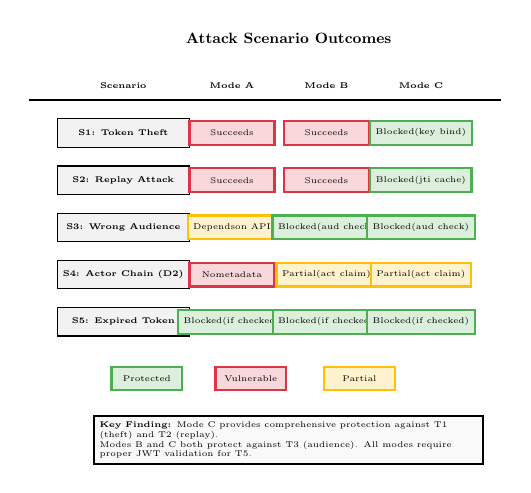
\begin{tikzpicture}[scale=0.6, every node/.style={scale=0.6}, font=\tiny]

\definecolor{failgreen}{RGB}{76,175,80}
\definecolor{successred}{RGB}{220,53,69}
\definecolor{partialyellow}{RGB}{255,193,7}

\tikzset{
    scenario/.style={rectangle, minimum width=2.8cm, minimum height=0.6cm,
                     text centered, draw=black, fill=gray!10, font=\tiny\bfseries},
    pass/.style={rectangle, minimum width=1.8cm, minimum height=0.5cm,
                 text centered, draw=failgreen, thick, fill=failgreen!20, font=\tiny},
    fail/.style={rectangle, minimum width=1.8cm, minimum height=0.5cm,
                 text centered, draw=successred, thick, fill=successred!20, font=\tiny},
    partial/.style={rectangle, minimum width=1.8cm, minimum height=0.5cm,
                    text centered, draw=partialyellow, thick, fill=partialyellow!20, font=\tiny},
}

% Title
\node[font=\small\bfseries] at (0,6) {Attack Scenario Outcomes};

% Column headers
\node[font=\tiny\bfseries] at (-3.5,5) {Scenario};
\node[font=\tiny\bfseries] at (-1.2,5) {Mode A};
\node[font=\tiny\bfseries] at (0.8,5) {Mode B};
\node[font=\tiny\bfseries] at (2.8,5) {Mode C};

% Horizontal line
\draw[thick] (-5.5,4.7) -- (4.5,4.7);

% S1: Token Theft
\node[scenario] (s1_label) at (-3.5,4) {S1: Token Theft};
\node[fail] (s1_a) at (-1.2,4) {Succeeds};
\node[fail] (s1_b) at (0.8,4) {Succeeds};
\node[pass] (s1_c) at (2.8,4) {Blocked\\(key bind)};

% S2: Replay Attack
\node[scenario] (s2_label) at (-3.5,3) {S2: Replay Attack};
\node[fail] (s2_a) at (-1.2,3) {Succeeds};
\node[fail] (s2_b) at (0.8,3) {Succeeds};
\node[pass] (s2_c) at (2.8,3) {Blocked\\(jti cache)};

% S3: Wrong Audience
\node[scenario] (s3_label) at (-3.5,2) {S3: Wrong Audience};
\node[partial] (s3_a) at (-1.2,2) {Depends\\on API};
\node[pass] (s3_b) at (0.8,2) {Blocked\\(aud check)};
\node[pass] (s3_c) at (2.8,2) {Blocked\\(aud check)};

% S4: Actor Chain
\node[scenario] (s4_label) at (-3.5,1) {S4: Actor Chain (D2)};
\node[fail] (s4_a) at (-1.2,1) {No\\metadata};
\node[partial] (s4_b) at (0.8,1) {Partial\\(act claim)};
\node[partial] (s4_c) at (2.8,1) {Partial\\(act claim)};

% S5: Expired Token
\node[scenario] (s5_label) at (-3.5,0) {S5: Expired Token};
\node[pass] (s5_a) at (-1.2,0) {Blocked\\(if checked)};
\node[pass] (s5_b) at (0.8,0) {Blocked\\(if checked)};
\node[pass] (s5_c) at (2.8,0) {Blocked\\(if checked)};

% Legend
\node[pass, minimum width=1.5cm] at (-3,-1.2) {Protected};
\node[fail, minimum width=1.5cm] at (-0.8,-1.2) {Vulnerable};
\node[partial, minimum width=1.5cm] at (1.5,-1.2) {Partial};

% Summary box
\node[rectangle, draw=black, thick, fill=gray!5, text width=8cm, font=\tiny, align=left] 
     at (0,-2.5) {
    \textbf{Key Finding:} Mode C provides comprehensive protection against T1 (theft) and T2 (replay).\\
    Modes B and C both protect against T3 (audience). All modes require proper JWT validation for T5.
};

\end{tikzpicture}

\caption{Attack scenario outcomes across authentication modes. Mode C blocks token theft (S1) and replay (S2), while Modes B and C both prevent audience misuse (S3).}
\label{tab:attacks}
\end{figure}

\section{Discussion}

\subsection{Interpretation of Results}

Our results show that layered authentication (Mode C) introduces measurable but acceptable latency overhead for ephemeral agent workloads. The median latency increase is on the order of 15.5 ms, which is tolerable for most internal service interactions. Caching dramatically reduces this overhead, making Mode C practical for agents that make multiple requests during their short lifetime.

The security gains are concrete. Mode C effectively blocks token theft (S1) and replay attacks (S2), two of the most common threats in bearer token systems. Token exchange (Modes B and C) improves audience validation and delegation traceability, addressing threats S3 and S4.

The throughput degradation at high churn (20 agents/second) suggests that Mode C may require additional infrastructure scaling (e.g., horizontal scaling of Keycloak, Redis clustering) in production environments with very high agent creation rates. However, for moderate churn (1--5 agents/second), the overhead is minimal.

\subsection{Limitations}

\textbf{Single-host deployment.} Our prototype runs on a single host, limiting the realism of network latency, distributed system failures, and cross-datacenter scenarios.

\textbf{Simplified threat model.} We do not address prompt injection, model-specific attacks, or compromised authorization servers. Our focus is narrowly on token-level authentication.

\textbf{Limited delegation depth.} We test only 1-hop and 2-hop delegation. Deeper delegation chains may introduce additional overhead and complexity.

\textbf{No formal verification.} Our evaluation is empirical. We do not provide formal proofs of security properties.

\textbf{Synthetic workload.} Our agents perform simple API calls. Real-world agents may have more complex workflows, longer lifetimes, or different request patterns.

\subsection{Deployment Considerations}

Practitioners considering layered authentication for ephemeral agents should consider:

\begin{itemize}
    \item \textbf{Cache strategy:} Token and key caching is essential for performance. Tokens should be cached within their validity period (e.g., 4 minutes for a 5-minute token), and keys should be reused across an agent's lifetime.
    \item \textbf{Replay cache placement:} Redis or equivalent replay cache should be co-located with the API service to minimize latency. Cache TTL should be set to token lifetime plus a small buffer.
    \item \textbf{Key rotation:} Ephemeral agents generate fresh key pairs on creation, providing natural key rotation. Long-lived agents may need explicit key rotation policies.
    \item \textbf{API verification cost:} DPoP verification adds CPU overhead for signature validation and replay cache lookup. APIs should optimize these operations (e.g., using efficient cryptographic libraries, batching cache lookups).
    \item \textbf{Scalability:} High churn rates may require horizontal scaling of the authorization server and replay cache. Load testing is recommended before production deployment.
\end{itemize}

\section{Conclusion}

This paper presents a focused empirical evaluation of layered authentication for ephemeral artificial intelligence agents. We implemented a reproducible prototype using token exchange, sender-constrained tokens, and replay protection, and compared it against simpler bearer-token baselines under varying agent churn, cache settings, and delegation depth.

Our results show that layered authentication (Mode C) introduces moderate latency overhead (\textbf{[PENDING]} ms median increase) but provides concrete security gains against token theft and replay attacks. Caching reduces this overhead by \textbf{[PENDING]}\%, making Mode C practical for agents that make multiple requests. Throughput degrades slightly at high churn (20 agents/second), suggesting the need for infrastructure scaling in high-volume scenarios.

The findings provide a compact evidence base for practitioners evaluating whether layered authentication is justified for their ephemeral agent workloads. For internal service interactions within a single trust domain, the security benefits of sender-constrained tokens and replay protection outweigh the performance costs, particularly when caching is enabled.

Future work should extend this evaluation to distributed deployments, deeper delegation chains, cross-domain federation, and integration with workload identity frameworks such as SPIFFE. Additionally, formal verification of the security properties of layered authentication compositions would complement this empirical study.

\section*{Acknowledgments}
\textit{Acknowledgments withheld for anonymous review.}

\bibliographystyle{IEEEtran}
\bibliography{references}

\end{document}
